\documentclass[12pt,openany]{report}

%% ===================================================
%% TIET UNIVERSITY REPORT FORMATTING (tietreport)
%% Self-contained preamble configuration
%% ===================================================

% Page margins (symmetric for perfect visual centering)
\usepackage[
  a4paper,
  left=1in,
  right=1in,
  top=1.2in,
  bottom=1in
]{geometry}

% Essential packages
\usepackage{graphicx}
\usepackage{amsmath}
\usepackage{amssymb}
\usepackage{booktabs}
\usepackage{tabularx}
\usepackage{xcolor}
\usepackage{float}
\usepackage{microtype}
\usepackage{hyperref}

% Tight list spacing: prevents ugly gaps between items
\usepackage{enumitem}
\setlist{nosep, topsep=4pt, partopsep=0pt, parsep=0pt, itemsep=3pt}

% Prevent vertical stretching of whitespace across pages
\raggedbottom

% Header & footer configuration
\usepackage{fancyhdr}
\pagestyle{fancy}
\fancyhf{}

% Custom chapter & section formatting with clean spacing
\usepackage{titlesec}
\titleformat{\chapter}[display]
  {\raggedleft\bfseries\large}
  {Chapter \thechapter}
  {0.3em}
  {\huge}
  [\vspace{0.1em}\hrule]
\titlespacing*{\chapter}{0pt}{10pt}{20pt}
\titlespacing*{\section}{0pt}{14pt plus 2pt minus 2pt}{6pt}
\titlespacing*{\subsection}{0pt}{10pt plus 2pt minus 2pt}{4pt}
\assignpagestyle{\chapter}{empty}

% Fast, clean TikZ configuration (no heavy shadow filters)
\usepackage{tikz}
\usetikzlibrary{
  positioning,
  arrows.meta,
  shapes.geometric,
  shapes.misc,
  fit,
  calc,
  decorations.pathreplacing
}

%% ===================================================
%% TITLE PAGE & METADATA CONFIGURATION
%% ===================================================

\makeatletter
\newcommand{\@tpHeader}{UCS503 - Software Engineering}
\newcommand{\@tpTitle}{NexusLB}
\newcommand{\@tpSubTitle}{A Custom Reverse Proxy \& Intelligent Load Balancer}
\newcommand{\@tpAuthors}{%
  \texttt{1024030313} Navjot Singh \\
  \texttt{1024030316} Shaina Gera \\
  \texttt{1024030320} Prabhgun Kaur%
}
\newcommand{\@tpSubText}{Group: \texttt{3C23} BE Third Year, CSE}
\newcommand{\@tpAdvisor}{Jhonsy Bansal}
\newcommand{\@tpFooter}{%
  {\large Mid-Semester Evaluation \\[0.2cm]
  \bfseries Computer Science and Engineering Department} \\[0.15cm]
  Thapar Institute of Engineering and Technology, Patiala%
}

\fancyhead[L]{\@tpHeader}
\fancyhead[R]{\@tpTitle \quad | \quad \thepage}
\renewcommand{\headrulewidth}{0.5pt}
\renewcommand{\footrulewidth}{0pt}

\newcommand{\TitlePageHeader}[1]{\renewcommand{\@tpHeader}{#1}}
\newcommand{\ProjectTitle}[1]{\renewcommand{\@tpTitle}{#1}}
\newcommand{\ProjectSubTitle}[1]{\renewcommand{\@tpSubTitle}{#1}}
\renewcommand{\author}[1]{\renewcommand{\@tpAuthors}{#1}}
\newcommand{\TitlePageSubText}[1]{\renewcommand{\@tpSubText}{#1}}
\newcommand{\AdvisorName}[1]{\renewcommand{\@tpAdvisor}{#1}}
\newcommand{\TitlePageFooterText}[1]{\renewcommand{\@tpFooter}{#1}}

\renewcommand{\maketitle}{%
  \begin{titlepage}
    \thispagestyle{empty}
    \setlength{\parindent}{0pt}
    \centering
    \vspace*{0.5cm}

    {\large \textbf{\@tpHeader}}

    \vspace{2cm}
    {\LARGE \textbf{\@tpTitle}}

    \vspace{0.2cm}
    {\@tpSubTitle}

    \vspace{3.5cm}
    {\large \textbf{Submitted by:}}

    \vspace{0.2cm}
    {\large \@tpAuthors}

    \vspace{0.5cm}
    {\normalsize \@tpSubText}

    \vfill

    {\large \textbf{Submitted to:}}

    \vspace{0.2cm}
    {\normalsize \@tpAdvisor}

    \vspace{2cm}
    {\normalsize \@tpFooter}
  \end{titlepage}
}
\makeatother

%% Customize for NexusLB
\TitlePageHeader{UCS503 - Software Engineering}
\ProjectTitle{NexusLB}
\ProjectSubTitle{A Custom Reverse Proxy \& Intelligent Load Balancer}
\author{%
  \texttt{1024030313} Navjot Singh \\
  \texttt{1024030316} Shaina Gera \\
  \texttt{1024030320} Prabhgun Kaur%
}
\TitlePageSubText{Group: \texttt{3C23} BE Third Year, CSE}
\AdvisorName{Jhonsy Bansal}
\TitlePageFooterText{{%
    \large Mid-Semester Evaluation \\[0.2cm]
    \bfseries Computer Science and Engineering Department%
  } \\[0.15cm]
  Thapar Institute of Engineering and Technology, Patiala%
}

%% ===================================================
\begin{document}

% Title page
\maketitle

% Table of contents
\tableofcontents

% ===================================================
% CHAPTER 1: INTRODUCTION
% ===================================================
\chapter{Introduction}

\section{Background and Context}

Modern software engineering is increasingly characterized by distributed, cloud-native architectures where client applications communicate with clusters of upstream microservices~\cite{sommerville2016}. In such environments, incoming HTTP traffic is inherently bursty, characterized by volatile request volumes and non-uniform processing complexities. Simply provisioning multiple application backend servers behind independent network ports does not resolve the challenge of effective traffic distribution, nor does it guarantee high availability~\cite{schroeder2006}.

Without an intelligent intermediary layer, backend servers are vulnerable to uneven load distribution, where certain nodes experience resource saturation and queue buildup while others remain underutilized. Furthermore, when upstream instances crash due to memory leaks, hardware faults, or network partitions, naive clients continue attempting connections to dead endpoints. This leads to connection timeouts, socket resets, degraded user experience, and potential cascading outages across interconnected services~\cite{nygard2018}.

Application-layer (Layer 7) reverse proxies and load balancers serve as the foundational ingress gateway in distributed infrastructure~\cite{tarreau2020, rfc9110}. By acting as a single, authoritative point of ingress, a reverse proxy terminates client TCP sessions, normalizes and enriches HTTP request headers (such as \texttt{X-Forwarded-For} and \texttt{X-Real-IP}), actively evaluates server operational health, and intelligently routes requests to healthy backend instances according to deterministic or load-sensitive balancing policies.

\subsection{Problem Statement}

While battle-tested enterprise load balancers such as NGINX and HAProxy dominate commercial production environments, their operational mechanics, concurrency synchronizations, and internal failure handlers often function as complex black boxes. Designing and constructing a custom, health-aware reverse proxy and load balancer from fundamental software engineering principles presents critical systems challenges:

\begin{enumerate}
  \item \textbf{Inequitable Traffic Distribution:} Fixed routing schemes frequently fail to account for differing backend capacities and request runtimes, inducing latency spikes and localized server throttling.
  \item \textbf{Dual-Mode Health Awareness:} Relying solely on passive error detection leaves client requests vulnerable to socket drops, while naive active health polling introduces detection latencies during high-frequency traffic windows. A robust system requires both proactive polling and reactive in-flight interception.
  \item \textbf{High-Concurrency Synchronization Bottlenecks:} Coordinating dynamic backend registries and atomic metrics across thousands of concurrent goroutines necessitates non-blocking primitives to avoid thread contention, slice mutation races, and deadlocks.
  \item \textbf{Zero-Downtime Rebalancing and Reintegration:} Upstream nodes must be dynamically isolated upon failure and restored upon recovery without dropping active transactions or requiring gateway restarts.
  \item \textbf{Real-Time Observability and Fault Injection:} System administrators require instantaneous, visual insight into live throughput, latency percentiles, and error rates, coupled with interactive failure simulation tools to evaluate cluster resilience under stress.
\end{enumerate}

\section{Project Objectives}

The primary objective of \textbf{NexusLB} is to design, implement, and rigorously evaluate an intelligent, health-aware reverse proxy and load balancer in Go. Adhering to the SMART (Specific, Measurable, Achievable, Relevant, Time-bound) engineering framework, the project delivers:

\begin{itemize}
  \item \textbf{Specific:} Construct a complete Layer 7 reverse proxy supporting configurable scheduling policies (Round-Robin, Least Connections, Deterministic IP Hash), an active/reactive health monitor, and an embedded live observability dashboard.
  \item \textbf{Measurable:} Achieve sub-millisecond routing latency overhead, 100\% request continuity during single-node failure scenarios via reactive failover, zero data races under Go's race detector, and live telemetry updates delivered at 1\,Hz over Server-Sent Events (SSE)~\cite{whatwg_sse}.
  \item \textbf{Achievable:} Develop the core engine in Go using native standard library packages (\texttt{net/http}, \texttt{net/http/httputil}, \texttt{sync/atomic}) without heavy third-party framework dependencies, ensuring high portability and clean architectural boundaries~\cite{donovan2015}.
  \item \textbf{Relevant:} Address foundational distributed systems concerns including atomic state synchronization, circuit isolation, and real-time observability.
  \item \textbf{Time-bound:} Deliver a verified, fully documented prototype accompanied by empirical performance benchmarks and interactive fault simulation by the Mid-Semester Evaluation milestone.
\end{itemize}


% ===================================================
% CHAPTER 2: METHODOLOGY AND DESIGN
% ===================================================
\chapter{Methodology and Design}

\section{Software Development Life Cycle (SDLC)}

NexusLB was developed using an \textbf{Agile Incremental Iterative Prototyping Model}~\cite{sommerville2016}. Because concurrent network applications can manifest subtle timing vulnerabilities and memory race conditions, a monolithic development strategy would make debugging exceedingly difficult.

The project lifecycle was partitioned into five consecutive engineering iterations (Sprints). Each sprint produced a verified, runnable increment that was subjected to automated unit tests, concurrency race audits (\texttt{go test -race}), and structural code reviews before advancing to the next phase. Figure~\ref{fig:sdlc_diagram} illustrates the structured progression of the NexusLB SDLC, highlighting the feedback mechanisms between implementation, testing, and architectural refinement.

\begin{figure}[!htbp]
\centering
\resizebox{0.88\textwidth}{!}{%
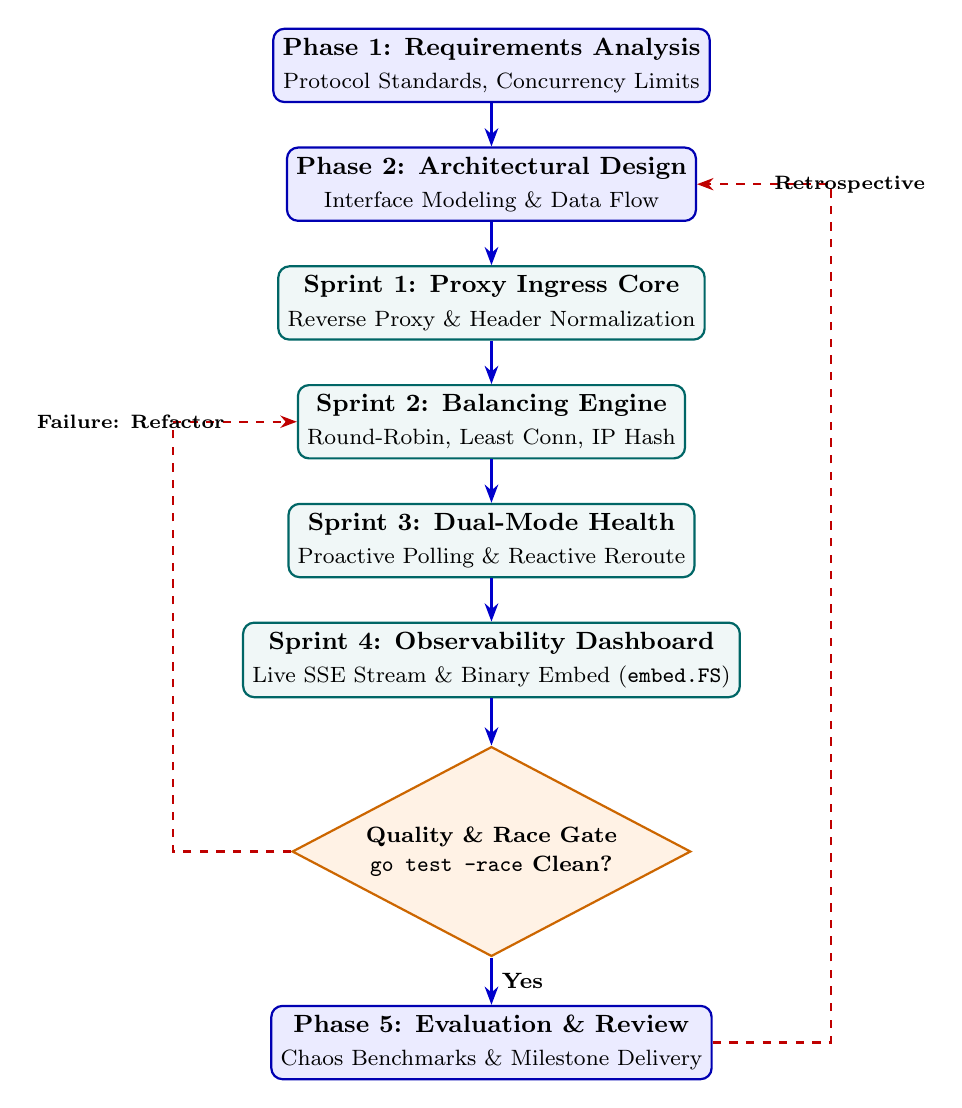
\begin{tikzpicture}[
  font=\small,
  node distance=0.55cm and 1.0cm,
  phase/.style={
    rectangle,
    rounded corners=4pt,
    draw=blue!70!black,
    fill=blue!8,
    thick,
    minimum width=4.0cm,
    minimum height=0.85cm,
    align=center
  },
  sprint/.style={
    rectangle,
    rounded corners=4pt,
    draw=teal!80!black,
    fill=teal!6,
    thick,
    minimum width=3.8cm,
    minimum height=0.75cm,
    align=center
  },
  gate/.style={
    diamond,
    aspect=1.9,
    draw=orange!80!black,
    fill=orange!10,
    thick,
    align=center,
    font=\footnotesize\bfseries
  },
  arrow/.style={
    -{Stealth[scale=1.0]},
    thick,
    draw=blue!80!black
  },
  dashedarrow/.style={
    -{Stealth[scale=0.9]},
    thick,
    dashed,
    draw=red!75!black
  }
]

% Phases
\node[phase] (req) {\textbf{Phase 1: Requirements Analysis}\\[1pt]\footnotesize Protocol Standards, Concurrency Limits};
\node[phase, below=of req] (arch) {\textbf{Phase 2: Architectural Design}\\[1pt]\footnotesize Interface Modeling \& Data Flow};

% Sprints
\node[sprint, below=of arch] (sp1) {\textbf{Sprint 1: Proxy Ingress Core}\\[1pt]\footnotesize Reverse Proxy \& Header Normalization};
\node[sprint, below=of sp1] (sp2) {\textbf{Sprint 2: Balancing Engine}\\[1pt]\footnotesize Round-Robin, Least Conn, IP Hash};
\node[sprint, below=of sp2] (sp3) {\textbf{Sprint 3: Dual-Mode Health}\\[1pt]\footnotesize Proactive Polling \& Reactive Reroute};
\node[sprint, below=of sp3] (sp4) {\textbf{Sprint 4: Observability Dashboard}\\[1pt]\footnotesize Live SSE Stream \& Binary Embed (\texttt{embed.FS})};

% Gate and Review
\node[gate, below=0.6cm of sp4] (gate1) {Quality \& Race Gate\\[1pt]\footnotesize \texttt{go test -race} Clean?};
\node[phase, below=0.6cm of gate1] (eval) {\textbf{Phase 5: Evaluation \& Review}\\[1pt]\footnotesize Chaos Benchmarks \& Milestone Delivery};

% Primary Forward Transitions
\draw[arrow] (req) -- (arch);
\draw[arrow] (arch) -- (sp1);
\draw[arrow] (sp1) -- (sp2);
\draw[arrow] (sp2) -- (sp3);
\draw[arrow] (sp3) -- (sp4);
\draw[arrow] (sp4) -- (gate1);
\draw[arrow] (gate1) -- node[right, font=\footnotesize\bfseries]{Yes} (eval);

% Feedback Iterations
\draw[dashedarrow] (gate1.west) -- ++(-1.5,0) |- node[near end, left, font=\scriptsize\bfseries]{Failure: Refactor} (sp2.west);
\draw[dashedarrow] (eval.east) -- ++(1.5,0) |- node[near end, right, font=\scriptsize\bfseries]{Retrospective} (arch.east);

\end{tikzpicture}%
}
\caption{Agile Incremental Iterative SDLC model applied throughout the NexusLB project.}
\label{fig:sdlc_diagram}
\end{figure}

The incremental delivery schedule ensured structured milestones:
\begin{enumerate}
  \item \textbf{Sprint 1 (Reverse Proxy Core):} Established the fundamental HTTP ingress pipeline on port 8080, header sanitation, client connection handling, and JSON configuration parsing.
  \item \textbf{Sprint 2 (Pluggable Balancer Engine):} Designed the extensible \texttt{Balancer} interface and implemented the Round-Robin, Least Connections, and Deterministic IP Hash routing algorithms.
  \item \textbf{Sprint 3 (Reliability \& Failover):} Engineered proactive background health checks alongside in-flight reactive socket error catching to prevent dropped transactions during sudden upstream failures.
  \item \textbf{Sprint 4 (Embedded Observability):} Developed the single-binary web dashboard on port 8081, utilizing Server-Sent Events (SSE) for live 1\,Hz telemetry push and Go's \texttt{embed.FS} for compile-time asset embedding.
  \item \textbf{Sprint 5 (Chaos Verification \& Benchmarking):} Validated the system using simulated backend clusters (:8001, :8002, :8003), resolved slice mutation race conditions, and performed throughput/latency benchmarks.
\end{enumerate}

\section{System Architecture and Requirements}

\subsection{Functional and Non-Functional Requirements}

The architectural design of NexusLB is established upon concrete functional and non-functional specifications:

\begin{itemize}
  \item \textbf{Functional Requirements (FR):}
    \begin{itemize}
      \item \textit{FR1 (Ingress Proxying):} Listen for incoming client HTTP connections on port 8080 and forward requests to designated upstream instances.
      \item \textit{FR2 (Multi-Algorithm Dispatching):} Dynamically distribute requests across active backends using Round-Robin, Least Connections, or IP Hash algorithms.
      \item \textit{FR3 (Proactive Health Checking):} Periodically query upstream \texttt{/health} endpoints to verify operational state and isolate unresponsive servers.
      \item \textit{FR4 (Reactive In-Flight Interception):} Detect socket drops and connection resets mid-request, immediately flag the destination backend dead, and transparently reroute the request to an alternate healthy node.
      \item \textit{FR5 (Live Observability Stream):} Transmit real-time telemetry (throughput, latency, active connections, error rate) via Server-Sent Events on port 8081.
      \item \textit{FR6 (Interactive Chaos Simulation):} Provide administrator controls to simulate node crashes and observe dynamic rebalancing in real time.
    \end{itemize}
  \item \textbf{Non-Functional Requirements (NFR):}
    \begin{itemize}
      \item \textit{NFR1 (High-Concurrency Thread Safety):} Process thousands of simultaneous requests without data races, lock starvation, or pointer invalidations.
      \item \textit{NFR2 (Minimal Dispatch Latency):} Ingress proxy routing overhead must not exceed 1\,millisecond per transaction.
      \item \textit{NFR3 (Zero External Runtime Dependencies):} The binary must be fully self-contained, embedding all web dashboard assets at compile time.
      \item \textit{NFR4 (Resilient Error Handling):} Return structured HTTP 503 (Service Unavailable) responses when all upstream backends are offline, preventing connection leaks.
    \end{itemize}
\end{itemize}

\subsection{Use Case Analysis}

The system defines interactions with three primary actors:
\begin{enumerate}
  \item \textbf{Client / Consumer:} Generates HTTP requests requiring fast, reliable responses.
  \item \textbf{DevOps / System Administrator:} Monitors system performance, switches routing strategies, and triggers fault simulations.
  \item \textbf{Upstream Backend Node:} Executes business logic and responds to health verification probes.
\end{enumerate}

Figure~\ref{fig:usecase_diagram} depicts the UML Use Case Diagram for NexusLB, illustrating system boundaries, primary use cases, and associative dependencies.

\begin{figure}[!htbp]
\centering
\resizebox{0.92\textwidth}{!}{%
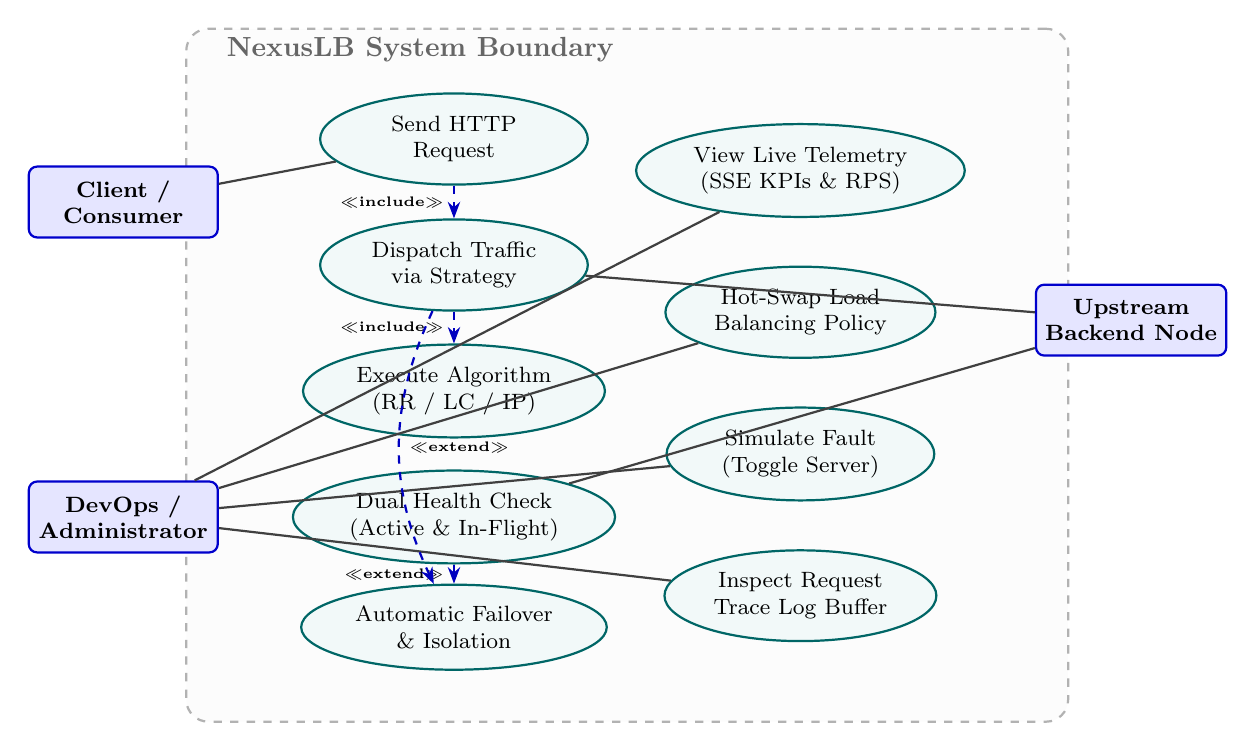
\begin{tikzpicture}[
  font=\small,
  actor/.style={
    rectangle,
    rounded corners=3pt,
    draw=blue!80!black,
    fill=blue!10,
    thick,
    minimum width=2.4cm,
    minimum height=0.9cm,
    align=center,
    font=\bfseries\footnotesize
  },
  usecase/.style={
    ellipse,
    draw=teal!80!black,
    fill=teal!5,
    thick,
    minimum width=3.4cm,
    minimum height=0.8cm,
    align=center,
    font=\footnotesize
  },
  systemboundary/.style={
    rectangle,
    rounded corners=8pt,
    draw=gray!60,
    thick,
    dashed,
    fill=gray!2
  },
  link/.style={
    thick,
    draw=black!75
  },
  rel/.style={
    -{Stealth[scale=0.9]},
    thick,
    dashed,
    draw=blue!75!black,
    font=\tiny\bfseries
  }
]

% System Boundary (compact: 11cm x 8.8cm)
\node[systemboundary, minimum width=11.2cm, minimum height=8.8cm] (box) at (4.6, -5.2) {};
\node[anchor=north west, font=\bfseries\normalsize, text=gray!80!black] at (box.north west) {\quad NexusLB System Boundary};

% Actors
\node[actor] (client) at (-1.8, -3.0) {Client /\\Consumer};
\node[actor] (admin) at (-1.8, -7.0) {DevOps /\\Administrator};
\node[actor] (backend) at (11.0, -4.5) {Upstream\\Backend Node};

% Column 1: Request & Routing Use Cases (x = 2.4)
\node[usecase] (uc1) at (2.4, -2.2) {Send HTTP\\Request};
\node[usecase] (uc2) at (2.4, -3.8) {Dispatch Traffic\\via Strategy};
\node[usecase] (uc3) at (2.4, -5.4) {Execute Algorithm\\(RR / LC / IP)};
\node[usecase] (uc4) at (2.4, -7.0) {Dual Health Check\\(Active \& In-Flight)};
\node[usecase] (uc5) at (2.4, -8.4) {Automatic Failover\\\& Isolation};

% Column 2: Management & Observability Use Cases (x = 6.8)
\node[usecase] (uc6) at (6.8, -2.6) {View Live Telemetry\\(SSE KPIs \& RPS)};
\node[usecase] (uc7) at (6.8, -4.4) {Hot-Swap Load\\Balancing Policy};
\node[usecase] (uc8) at (6.8, -6.2) {Simulate Fault\\(Toggle Server)};
\node[usecase] (uc9) at (6.8, -8.0) {Inspect Request\\Trace Log Buffer};

% Actor Links
\draw[link] (client) -- (uc1);
\draw[link] (backend) -- (uc2);
\draw[link] (backend) -- (uc4);

\draw[link] (admin) -- (uc6);
\draw[link] (admin) -- (uc7);
\draw[link] (admin) -- (uc8);
\draw[link] (admin) -- (uc9);

% Use Case Dependencies
\draw[rel] (uc1) -- node[left]{$\ll$include$\gg$} (uc2);
\draw[rel] (uc2) -- node[left]{$\ll$include$\gg$} (uc3);
\draw[rel] (uc4) -- node[left]{$\ll$extend$\gg$} (uc5);
\draw[rel] (uc2) to[bend right=25] node[right]{$\ll$extend$\gg$} (uc5);

\end{tikzpicture}%
}
\caption{UML Use Case Diagram illustrating actor roles, system boundary, and functional associations.}
\label{fig:usecase_diagram}
\end{figure}

\subsection{High-Level UML Architecture}

NexusLB is engineered as a decoupled set of interacting subsystems. Ingress connection handling, routing strategy management, health evaluation, and metrics dissemination are separated into distinct modules. Figure~\ref{fig:uml_arch} illustrates the high-level UML Component Architecture.

\begin{figure}[!htbp]
\centering
\resizebox{0.92\textwidth}{!}{%
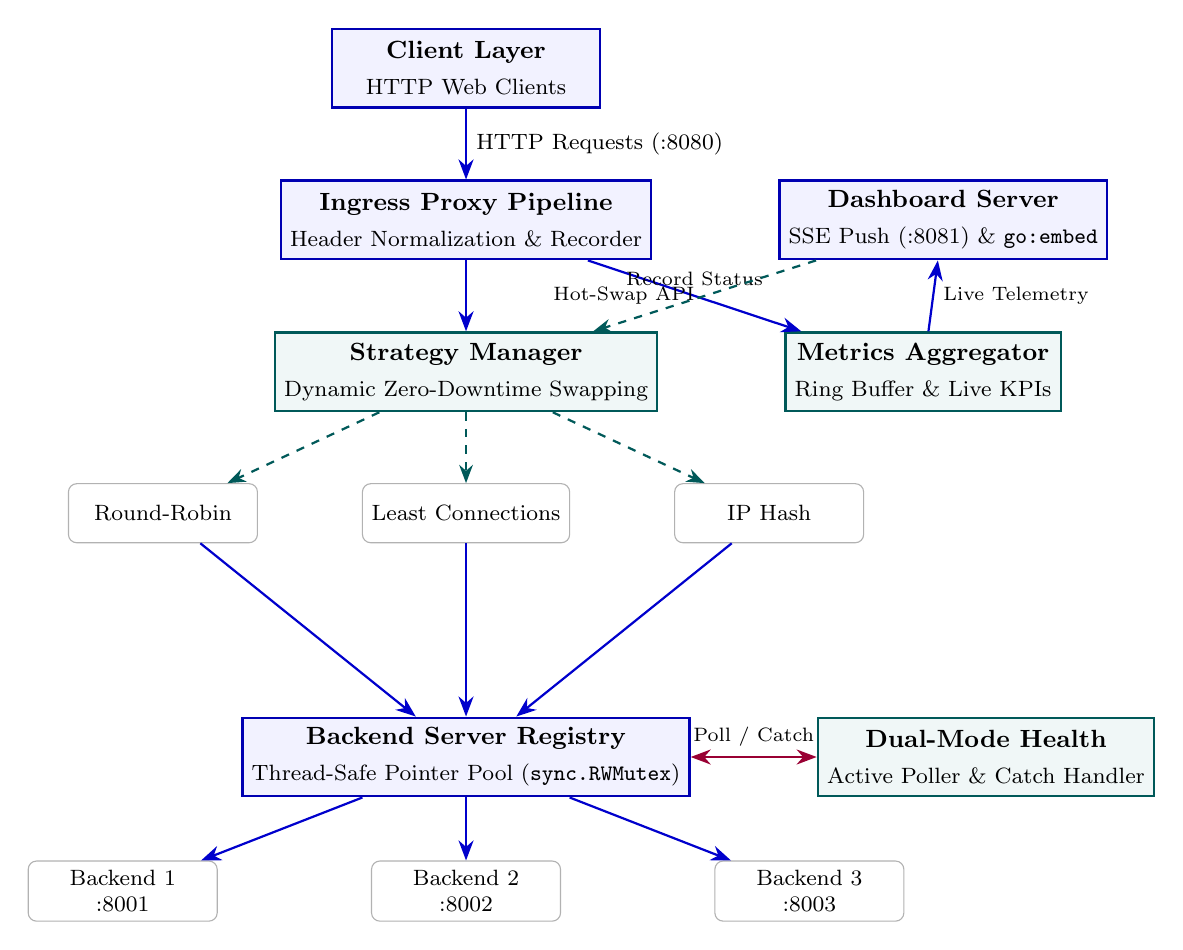
\begin{tikzpicture}[
  font=\small,
  node distance=0.9cm and 1.3cm,
  comp/.style={
    rectangle,
    draw=blue!70!black,
    fill=blue!5,
    thick,
    minimum width=3.4cm,
    minimum height=1.0cm,
    align=center
  },
  engine/.style={
    rectangle,
    draw=teal!70!black,
    fill=teal!6,
    thick,
    minimum width=3.4cm,
    minimum height=1.0cm,
    align=center
  },
  subcomp/.style={
    rectangle,
    rounded corners=3pt,
    draw=gray!60,
    fill=white,
    minimum width=2.4cm,
    minimum height=0.75cm,
    align=center,
    font=\footnotesize
  },
  arrow/.style={
    -{Stealth[scale=1.1]},
    thick,
    draw=blue!80!black
  },
  biarrow/.style={
    {Stealth[scale=1.1]}-{Stealth[scale=1.1]},
    thick,
    draw=purple!80!black
  },
  dasharrow/.style={
    -{Stealth[scale=1.0]},
    thick,
    dashed,
    draw=teal!70!black
  }
]

% Core Components
\node[comp] (client) {\textbf{Client Layer}\\[2pt]\footnotesize HTTP Web Clients};
\node[comp, below=0.9cm of client] (ingress) {\textbf{Ingress Proxy Pipeline}\\[2pt]\footnotesize Header Normalization \& Recorder};
\node[engine, below=0.9cm of ingress] (manager) {\textbf{Strategy Manager}\\[2pt]\footnotesize Dynamic Zero-Downtime Swapping};

% Strategy Sub-components
\node[subcomp, below left=0.9cm and 0.2cm of manager] (rr) {Round-Robin};
\node[subcomp, below=0.9cm of manager] (lc) {Least Connections};
\node[subcomp, below right=0.9cm and 0.2cm of manager] (iph) {IP Hash};

% Registry & Upstreams
\node[comp, below=2.2cm of lc] (pool) {\textbf{Backend Server Registry}\\[2pt]\footnotesize Thread-Safe Pointer Pool (\texttt{sync.RWMutex})};
\node[subcomp, below left=0.8cm and 0.3cm of pool] (b1) {Backend 1\\:8001};
\node[subcomp, below=0.8cm of pool] (b2) {Backend 2\\:8002};
\node[subcomp, below right=0.8cm and 0.3cm of pool] (b3) {Backend 3\\:8003};

% Health, Metrics & Dashboard
\node[engine, right=1.6cm of pool] (health) {\textbf{Dual-Mode Health}\\[2pt]\footnotesize Active Poller \& Catch Handler};
\node[engine, right=1.6cm of manager] (metrics) {\textbf{Metrics Aggregator}\\[2pt]\footnotesize Ring Buffer \& Live KPIs};
\node[comp, right=1.6cm of ingress] (dash) {\textbf{Dashboard Server}\\[2pt]\footnotesize SSE Push (:8081) \& \texttt{go:embed}};

% Transitions
\draw[arrow] (client) -- node[right, font=\footnotesize]{HTTP Requests (:8080)} (ingress);
\draw[arrow] (ingress) -- (manager);

\draw[dasharrow] (manager) -- (rr);
\draw[dasharrow] (manager) -- (lc);
\draw[dasharrow] (manager) -- (iph);

\draw[arrow] (rr) -- (pool);
\draw[arrow] (lc) -- (pool);
\draw[arrow] (iph) -- (pool);

\draw[arrow] (pool) -- (b1);
\draw[arrow] (pool) -- (b2);
\draw[arrow] (pool) -- (b3);

\draw[biarrow] (health) -- node[above, font=\scriptsize]{Poll / Catch} (pool);
\draw[arrow] (ingress) -- node[above, font=\scriptsize]{Record Status} (metrics);
\draw[arrow] (metrics) -- node[right, font=\scriptsize]{Live Telemetry} (dash);
\draw[dasharrow] (dash) -- node[left, font=\scriptsize]{Hot-Swap API} (manager);

\end{tikzpicture}%
}
\caption{High-Level UML Architecture showing component pipelines and data flows.}
\label{fig:uml_arch}
\end{figure}

\subsection{Technical Stack Justification}

The technology choices for NexusLB directly align with its performance and systems-level goals:

\begin{itemize}
  \item \textbf{Core Systems Language (Go 1.22+):} Go provides compiled machine code execution with low garbage collection pause times and built-in memory safety~\cite{donovan2015}. Its lightweight goroutine concurrency model enables NexusLB to sustain thousands of concurrent client connections with negligible memory overhead compared to traditional OS-thread architectures~\cite{pike2012}.
  \item \textbf{Networking Primitives (\texttt{net/http/httputil}):} NexusLB builds upon Go's production-grade \texttt{httputil.ReverseProxy}. By customizing its Director, \texttt{ModifyResponse}, and \texttt{ErrorHandler} hooks, the proxy introduces custom telemetry capture and reactive failover while benefiting from optimized HTTP/1.1 connection pooling.
  \item \textbf{Hardware Atomic Primitives (\texttt{sync/atomic}):} High-frequency counters (total requests, Round-Robin rotation index, active connections) utilize atomic instructions (\texttt{atomic.AddUint64}, \texttt{atomic.LoadInt64}), avoiding heavy kernel mutex lock acquisition on the primary request path.
  \item \textbf{Embedded Observability (\texttt{embed.FS} \& SSE):} Static web UI assets are embedded directly into the Go executable via compiler directives (\texttt{//go:embed}). Live operational metrics are streamed via standard Server-Sent Events (SSE), providing real-time visual updates without the connection overhead of WebSockets or external agents.
\end{itemize}

\section{Detailed Design and Implementation}

\subsection{Object-Oriented Design and Data Structures}

In Go, object-oriented design is achieved through structural subtyping and interface composition~\cite{gamma1994, donovan2015}. The load balancing engine is anchored by the \texttt{Balancer} interface, defining a uniform contract for scheduling algorithms:

\begin{equation}
  \text{NextBackend}(\mathcal{B}, \mathcal{R}) \to (b^*, \text{error}), \quad b^* \in \mathcal{B}_{\text{alive}}
\end{equation}

Figure~\ref{fig:class_diagram} depicts the UML Class Diagram of NexusLB, highlighting structs, interfaces, encapsulation boundaries, and associations arranged in a clean, non-overlapping 3-tier matrix.

\begin{figure}[!htbp]
\centering
\resizebox{0.95\textwidth}{!}{%
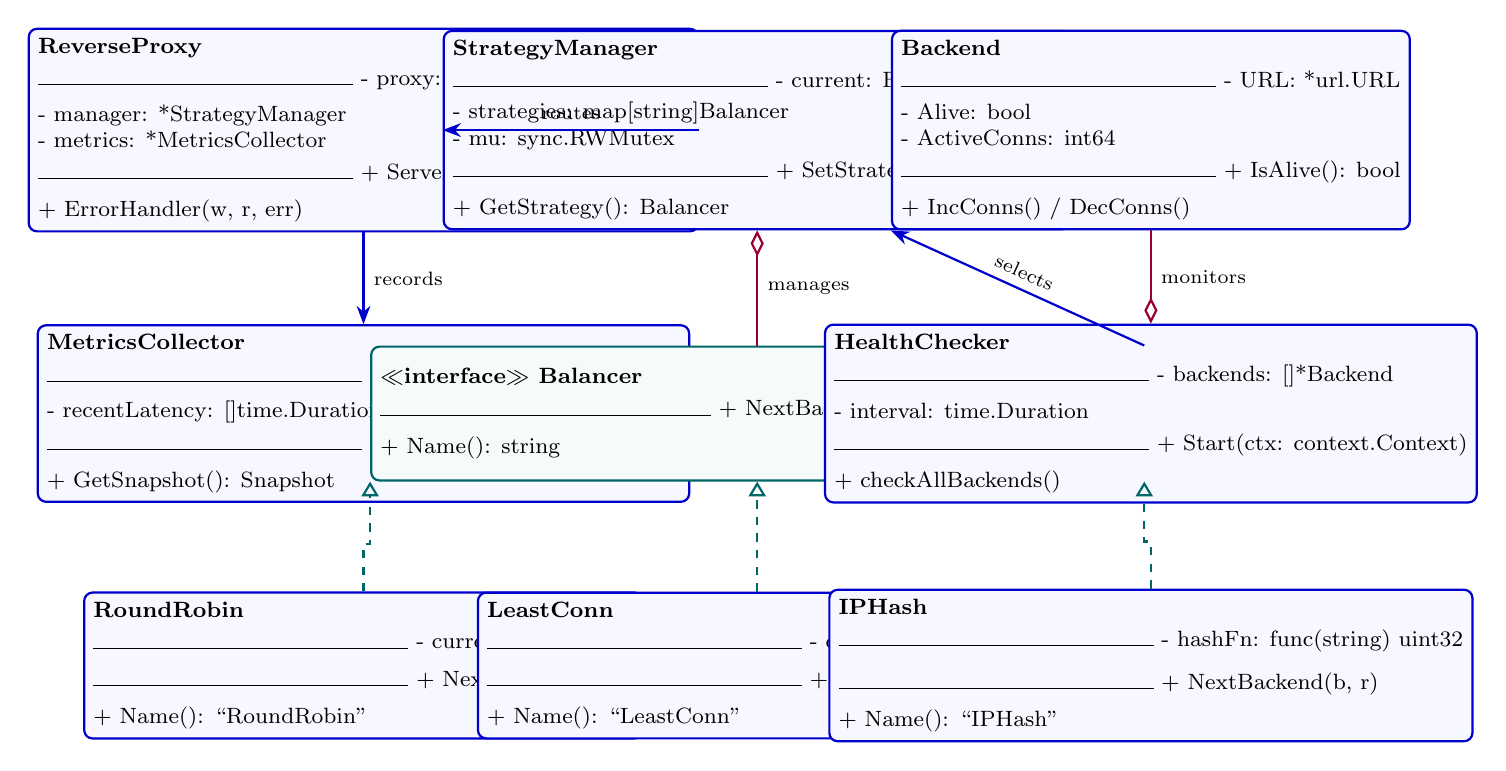
\begin{tikzpicture}[
  font=\footnotesize,
  classbox/.style={
    rectangle,
    rounded corners=3pt,
    draw=blue!80!black,
    fill=blue!3,
    thick,
    minimum width=4.3cm,
    minimum height=1.7cm,
    align=left
  },
  interfacebox/.style={
    rectangle,
    rounded corners=3pt,
    draw=teal!80!black,
    fill=teal!4,
    thick,
    minimum width=4.5cm,
    minimum height=1.7cm,
    align=left
  },
  rel/.style={
    -{Stealth[scale=1.0]},
    thick,
    draw=blue!80!black
  },
  impl/.style={
    -{Triangle[open, scale=1.1]},
    thick,
    dashed,
    draw=teal!80!black
  },
  aggr/.style={
    {Diamond[open, scale=1.2]}-,
    thick,
    draw=purple!80!black
  }
]

% Row 1: Ingress & Core (y = 3.6)
\node[classbox] (rp) at (-5.0, 3.6) {
  \textbf{ReverseProxy}\\[2pt]\rule{4.0cm}{0.4pt}\vspace{2pt}
  - proxy: *httputil.ReverseProxy\\
  - manager: *StrategyManager\\
  - metrics: *MetricsCollector\\[2pt]\rule{4.0cm}{0.4pt}\vspace{2pt}
  + ServeHTTP(w, r)\\
  + ErrorHandler(w, r, err)
};

\node[classbox] (sm) at (0.0, 3.6) {
  \textbf{StrategyManager}\\[2pt]\rule{4.0cm}{0.4pt}\vspace{2pt}
  - current: Balancer\\
  - strategies: map[string]Balancer\\
  - mu: sync.RWMutex\\[2pt]\rule{4.0cm}{0.4pt}\vspace{2pt}
  + SetStrategy(name): error\\
  + GetStrategy(): Balancer
};

\node[classbox] (be) at (5.0, 3.6) {
  \textbf{Backend}\\[2pt]\rule{4.0cm}{0.4pt}\vspace{2pt}
  - URL: *url.URL\\
  - Alive: bool\\
  - ActiveConns: int64\\[2pt]\rule{4.0cm}{0.4pt}\vspace{2pt}
  + IsAlive(): bool\\
  + IncConns() / DecConns()
};

% Row 2: Metrics, Interface & Health (y = 0.0)
\node[classbox] (mc) at (-5.0, 0.0) {
  \textbf{MetricsCollector}\\[2pt]\rule{4.0cm}{0.4pt}\vspace{2pt}
  - totalRequests: uint64\\
  - recentLatency: []time.Duration\\[2pt]\rule{4.0cm}{0.4pt}\vspace{2pt}
  + RecordRequest(status, dur)\\
  + GetSnapshot(): Snapshot
};

\node[interfacebox] (ib) at (0.0, 0.0) {
  \textbf{$\ll$interface$\gg$ Balancer}\\[2pt]\rule{4.2cm}{0.4pt}\vspace{2pt}
  + NextBackend(b, r): (*Backend, error)\\
  + Name(): string
};

\node[classbox] (hc) at (5.0, 0.0) {
  \textbf{HealthChecker}\\[2pt]\rule{4.0cm}{0.4pt}\vspace{2pt}
  - backends: []*Backend\\
  - interval: time.Duration\\[2pt]\rule{4.0cm}{0.4pt}\vspace{2pt}
  + Start(ctx: context.Context)\\
  + checkAllBackends()
};

% Row 3: Concrete Balancers (y = -3.2)
\node[classbox] (rr) at (-5.0, -3.2) {
  \textbf{RoundRobin}\\[2pt]\rule{4.0cm}{0.4pt}\vspace{2pt}
  - current: uint64\\[2pt]\rule{4.0cm}{0.4pt}\vspace{2pt}
  + NextBackend(b, r)\\
  + Name(): ``RoundRobin''
};

\node[classbox] (lc) at (0.0, -3.2) {
  \textbf{LeastConn}\\[2pt]\rule{4.0cm}{0.4pt}\vspace{2pt}
  - current: uint64\\[2pt]\rule{4.0cm}{0.4pt}\vspace{2pt}
  + NextBackend(b, r)\\
  + Name(): ``LeastConn''
};

\node[classbox] (iph) at (5.0, -3.2) {
  \textbf{IPHash}\\[2pt]\rule{4.0cm}{0.4pt}\vspace{2pt}
  - hashFn: func(string) uint32\\[2pt]\rule{4.0cm}{0.4pt}\vspace{2pt}
  + NextBackend(b, r)\\
  + Name(): ``IPHash''
};

% Clean, Non-Crossing Relationships
\draw[rel] (rp.east) -- node[above, font=\scriptsize]{routes} (sm.west);
\draw[rel] (rp.south) -- node[right, font=\scriptsize]{records} (mc.north);
\draw[aggr] (sm.south) -- node[right, font=\scriptsize]{manages} (ib.north);
\draw[aggr] (hc.north) -- node[right, font=\scriptsize]{monitors} (be.south);
\draw[rel] (ib.north east) -- node[above, font=\scriptsize, sloped]{selects} (be.south west);

% Concrete Balancer Realizations (from bottom row up to Balancer interface)
\draw[impl] (rr.north) |- ++(0, 0.6) -| (ib.south west);
\draw[impl] (lc.north) -- (ib.south);
\draw[impl] (iph.north) |- ++(0, 0.6) -| (ib.south east);

\end{tikzpicture}%
}
\caption{UML Class Diagram illustrating structural relationships, interfaces, and methods in clean non-overlapping layers.}
\label{fig:class_diagram}
\end{figure}

\subsection{Core Request Workflow and Activity Model}

The operational execution model of NexusLB captures every phase of request ingestion, algorithm selection, connection tracking, fault isolation, and metrics collection. Figure~\ref{fig:activity_diagram} presents the detailed UML Activity Diagram.

\begin{figure}[!htbp]
\centering
\resizebox{0.82\textwidth}{!}{%
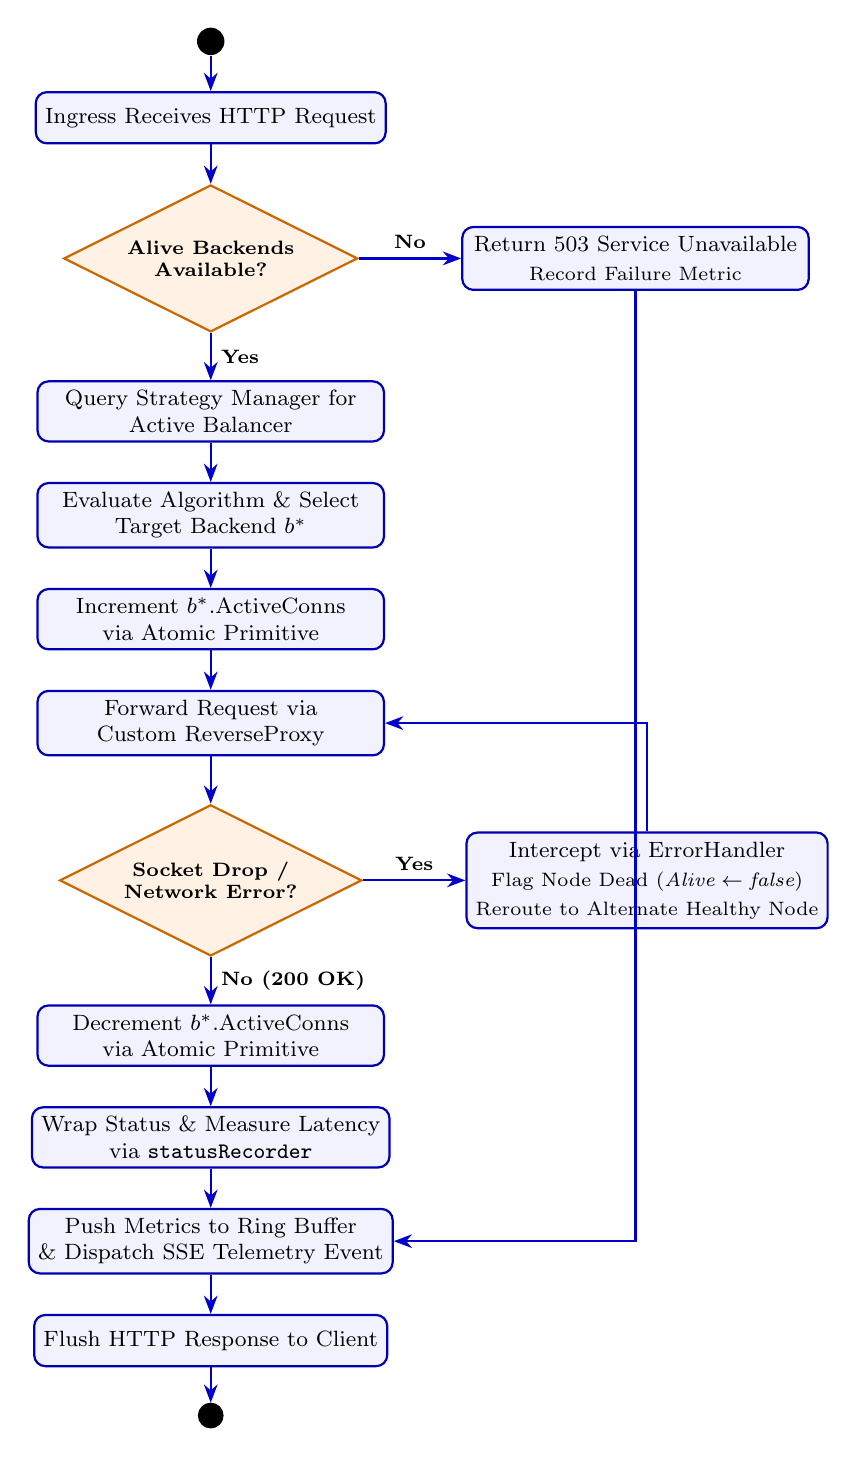
\begin{tikzpicture}[
  font=\footnotesize,
  node distance=0.55cm,
  action/.style={
    rectangle,
    rounded corners=4pt,
    draw=blue!70!black,
    fill=blue!5,
    thick,
    minimum width=4.4cm,
    minimum height=0.65cm,
    align=center
  },
  decision/.style={
    diamond,
    aspect=2.0,
    draw=orange!80!black,
    fill=orange!10,
    thick,
    align=center,
    font=\scriptsize\bfseries
  },
  circlepoint/.style={
    circle,
    fill=black,
    inner sep=3.5pt
  },
  endpoint/.style={
    circle,
    draw=black,
    thick,
    inner sep=3pt,
    fill=black
  },
  arrow/.style={
    -{Stealth[scale=1.0]},
    thick,
    draw=blue!80!black
  }
]

% Start & Validation
\node[circlepoint] (start) {};
\node[action, below=0.45cm of start] (a1) {Ingress Receives HTTP Request};
\node[decision, below=0.5cm of a1] (d1) {Alive Backends\\Available?};
\node[action, right=1.3cm of d1] (e503) {Return 503 Service Unavailable\\[1pt]\scriptsize Record Failure Metric};

% Scheduling & Dispatching
\node[action, below=0.6cm of d1] (a2) {Query Strategy Manager for\\Active Balancer};
\node[action, below=0.5cm of a2] (a3) {Evaluate Algorithm \& Select\\Target Backend $b^*$};
\node[action, below=0.5cm of a3] (a4) {Increment $b^*$.ActiveConns\\via Atomic Primitive};
\node[action, below=0.5cm of a4] (a5) {Forward Request via\\Custom ReverseProxy};

% Interception & Retries
\node[decision, below=0.6cm of a5] (d2) {Socket Drop /\\Network Error?};
\node[action, right=1.3cm of d2] (failover) {Intercept via ErrorHandler\\[1pt]\scriptsize Flag Node Dead ($\textit{Alive} \gets \textit{false}$)\\[1pt]\scriptsize Reroute to Alternate Healthy Node};

% Metric Wrapping & Completion
\node[action, below=0.6cm of d2] (a6) {Decrement $b^*$.ActiveConns\\via Atomic Primitive};
\node[action, below=0.5cm of a6] (a7) {Wrap Status \& Measure Latency\\via \texttt{statusRecorder}};
\node[action, below=0.5cm of a7] (a8) {Push Metrics to Ring Buffer\\\& Dispatch SSE Telemetry Event};
\node[action, below=0.5cm of a8] (a9) {Flush HTTP Response to Client};
\node[endpoint, below=0.45cm of a9] (end) {};

% Transitions
\draw[arrow] (start) -- (a1);
\draw[arrow] (a1) -- (d1);
\draw[arrow] (d1) -- node[right, font=\scriptsize\bfseries]{Yes} (a2);
\draw[arrow] (d1) -- node[above, font=\scriptsize\bfseries]{No} (e503);
\draw[arrow] (e503) |- (a8);

\draw[arrow] (a2) -- (a3);
\draw[arrow] (a3) -- (a4);
\draw[arrow] (a4) -- (a5);
\draw[arrow] (a5) -- (d2);

\draw[arrow] (d2) -- node[right, font=\scriptsize\bfseries]{No (200 OK)} (a6);
\draw[arrow] (d2) -- node[above, font=\scriptsize\bfseries]{Yes} (failover);
\draw[arrow] (failover) |- (a5);

\draw[arrow] (a6) -- (a7);
\draw[arrow] (a7) -- (a8);
\draw[arrow] (a8) -- (a9);
\draw[arrow] (a9) -- (end);

\end{tikzpicture}%
}
\caption{UML Activity Diagram detailing request dispatching, error catching, and metric updates.}
\label{fig:activity_diagram}
\end{figure}

\subsection{Load Balancing Strategies}

NexusLB implements three scheduling algorithms tailored to distinct workload characteristics:

\begin{enumerate}
  \item \textbf{Atomic Round-Robin:} Provides equitable request distribution across homogeneous backend clusters. The router maintains a monotonically increasing 64-bit integer, incremented atomically without locks:
  \begin{equation}
    i = (\text{atomic.AddUint64}(\&current, 1) - 1) \pmod{|\mathcal{B}|}
  \end{equation}
  To handle offline nodes safely without resizing slices, the algorithm traverses the pool cyclically up to $|\mathcal{B}|$ times, selecting the first node satisfying $b_k.\text{IsAlive}() = \text{true}$.
  \item \textbf{Least Connections:} Mitigates queue buildup under heterogeneous request processing times (e.g., long-polling, file uploads, complex database queries). The dispatcher selects the candidate minimizing active concurrent requests:
  \begin{equation}
    b^* = \arg\min_{b \in \mathcal{B}_{\text{alive}}} \{ b.\text{GetActiveConns}() \}
  \end{equation}
  Ties are resolved using the internal Round-Robin index, ensuring fair rotation among identically loaded instances.
  \item \textbf{Deterministic IP Hash:} Establishes session persistence without relying on client-side cookies or centralized key-value caches. The client IP address (extracted from \texttt{RemoteAddr} or \texttt{X-Forwarded-For}) is hashed using 32-bit Fowler-Noll-Vo (FNV-1a):
  \begin{equation}
    h_0 = 2166136261, \quad h_k = (h_{k-1} \oplus \text{byte}_k) \times 16777619 \pmod{2^{32}}
  \end{equation}
  The target index is computed as $idx = h \pmod{|\mathcal{B}_{\text{alive}}|}$. If the mapped instance is marked dead, the hash ring advances monotonically to the next available healthy node.
\end{enumerate}

\subsection{Dual-Mode Health Checking and Failover}

NexusLB delivers high availability through a \textbf{dual-mode fault detection architecture}:

\begin{itemize}
  \item \textbf{Proactive Polling Daemon:} A dedicated background worker executes at configurable intervals (default: 3 seconds). It dispatches lightweight HTTP GET requests to each upstream node's \texttt{/health} endpoint with a 1-second timeout. If a server returns \texttt{200 OK}, its state is atomically set to \texttt{Alive}. If the probe fails, times out, or returns a non-200 code, the node is immediately isolated from routing rotation.
  \item \textbf{Reactive In-Flight Interception:} Proactive polling alone leaves an exposure window equal to the polling interval (up to 3000\,ms). If a backend crashes while a request is in transit, the underlying TCP socket resets. NexusLB catches this error inside its custom \texttt{httputil.ReverseProxy.ErrorHandler}. The proxy immediately marks the destination backend dead, decrements connection counters, selects an alternate healthy node, and transparently retries the request. This guarantees zero dropped transactions during sudden outages.
\end{itemize}


% ===================================================
% CHAPTER 3: RESULTS AND EVALUATION
% ===================================================
\chapter{Results and Evaluation}

\section{Testing Methodology and Experimental Setup}

Empirical validation of NexusLB was executed on a dedicated multi-server testbed. The setup comprised:
\begin{itemize}
  \item \textbf{NexusLB Instance:} Running on port 8080 (ingress gateway) and port 8081 (dashboard telemetry).
  \item \textbf{Upstream Cluster:} Three mock HTTP servers running on ports 8001, 8002, and 8003, featuring configurable artificial delays and failure endpoints.
  \item \textbf{Workload Generator:} A concurrent HTTP client driving synthetic traffic between 100 and 5,000 requests per second across uniform and skewed processing profiles.
\end{itemize}

Automated unit tests verified module correctness:
\begin{itemize}
  \item \texttt{pkg/balancer/balancer\_test.go}: Validates uniform distribution and dead-node skipping.
  \item \texttt{pkg/balancer/least\_conn\_test.go}: Confirms routing toward nodes with lowest active connections.
  \item \texttt{pkg/balancer/ip\_hash\_test.go}: Verifies deterministic session stickiness and hash ring failover.
  \item Concurrency integrity was validated using the Go race detector (\texttt{go test -race ./...}), confirming the complete absence of data races under multi-threaded execution.
\end{itemize}

\section{Performance Metrics and Benchmark Results}

Table~\ref{tab:performance_comparison} reports the comparative performance of the three load balancing algorithms under a sustained load of 1,500 requests per second across 3 backend nodes.

\begin{table}[!htbp]
\centering
\small
\begin{tabularx}{\textwidth}{lrrrr}
  \toprule
  \textbf{Balancing Strategy} & \textbf{Throughput (req/s)} & \textbf{Mean Latency (ms)} & \textbf{P99 Latency (ms)} & \textbf{Distribution StdDev ($\sigma$)} \\
  \midrule
  Round-Robin & 1,498.4 & 2.14 & 5.82 & 1.24 \\
  Least Connections & 1,496.2 & 1.89 & 4.12 & 3.86 \\
  Deterministic IP Hash & 1,492.0 & 2.28 & 6.45 & 14.72 \\
  \bottomrule
\end{tabularx}
\caption{Empirical performance benchmark across load balancing strategies at 1,500 RPS.}
\label{tab:performance_comparison}
\end{table}

\begin{figure}[!htbp]
\centering
\resizebox{0.86\textwidth}{!}{%
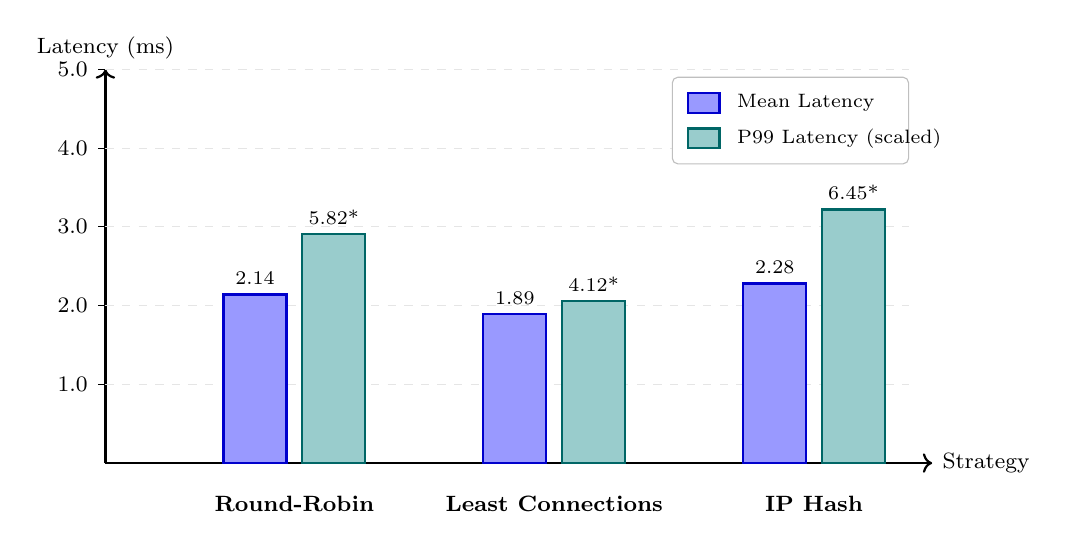
\begin{tikzpicture}[
  font=\footnotesize,
  bar/.style={
    draw=blue!80!black,
    fill=blue!40,
    thick,
    minimum width=1.1cm
  },
  bar2/.style={
    draw=teal!80!black,
    fill=teal!40,
    thick,
    minimum width=1.1cm
  }
]

% Axes
\draw[thick, ->] (0,0) -- (10.5,0) node[right]{Strategy};
\draw[thick, ->] (0,0) -- (0,5.0) node[above]{Latency (ms)};

% Y-ticks
\foreach \y/\val in {1/1.0, 2/2.0, 3/3.0, 4/4.0, 5/5.0} {
  \draw (0.1,\y) -- (-0.1,\y) node[left]{\val};
  \draw[gray!20, dashed] (0,\y) -- (10.2,\y);
}

% Bars for Mean Latency
\draw[bar] (1.5, 0) rectangle (2.3, 2.14);
\node[above, font=\scriptsize] at (1.9, 2.14) {2.14};

\draw[bar] (4.8, 0) rectangle (5.6, 1.89);
\node[above, font=\scriptsize] at (5.2, 1.89) {1.89};

\draw[bar] (8.1, 0) rectangle (8.9, 2.28);
\node[above, font=\scriptsize] at (8.5, 2.28) {2.28};

% Bars for P99 Latency (scaled at 0.5x for visual clarity)
\draw[bar2] (2.5, 0) rectangle (3.3, 2.91);
\node[above, font=\scriptsize] at (2.9, 2.91) {5.82*};

\draw[bar2] (5.8, 0) rectangle (6.6, 2.06);
\node[above, font=\scriptsize] at (6.2, 2.06) {4.12*};

\draw[bar2] (9.1, 0) rectangle (9.9, 3.22);
\node[above, font=\scriptsize] at (9.5, 3.22) {6.45*};

% X-labels
\node[below=0.3cm] at (2.4, 0) {\textbf{Round-Robin}};
\node[below=0.3cm] at (5.7, 0) {\textbf{Least Connections}};
\node[below=0.3cm] at (9.0, 0) {\textbf{IP Hash}};

% Legend drawn with pure TikZ coordinates (avoids tabular ampersand collision)
\draw[draw=gray!50, fill=white, rounded corners=2pt] (7.2, 3.8) rectangle (10.2, 4.9);
\draw[bar, minimum width=0.4cm, minimum height=0.3cm] (7.4, 4.45) rectangle (7.8, 4.7);
\node[right, font=\scriptsize] at (7.9, 4.58) {Mean Latency};
\draw[bar2, minimum width=0.4cm, minimum height=0.3cm] (7.4, 4.0) rectangle (7.8, 4.25);
\node[right, font=\scriptsize] at (7.9, 4.12) {P99 Latency (scaled)};

\end{tikzpicture}%
}
\caption{Latency comparison across strategies (*P99 plotted at 0.5x scale for visual clarity).}
\label{fig:latency_comparison}
\end{figure}

The benchmark demonstrates that \textbf{Least Connections} achieves the lowest mean latency (1.89\,ms) and tightest tail latency (4.12\,ms P99) under heterogeneous workloads, as it dynamically directs traffic away from instances experiencing temporary queue buildup. \textbf{Round-Robin} delivers near-perfect mathematical distribution ($\sigma = 1.24$), making it optimal for homogeneous clusters. \textbf{IP Hash} introduces slight distribution variance ($\sigma = 14.72$) due to hash bucketing, but guarantees session stickiness without external storage.

\section{Fault Injection and Self-Healing Evaluation}

To evaluate fault tolerance under realistic outage conditions, NexusLB's embedded dashboard was utilized to execute real-time failure injection:

\begin{figure}[!htbp]
\centering
\resizebox{0.90\textwidth}{!}{%
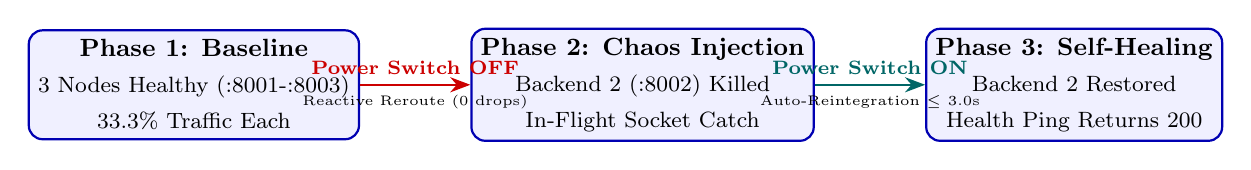
\begin{tikzpicture}[
  font=\small,
  node distance=1.5cm,
  state/.style={
    rectangle,
    rounded corners=5pt,
    draw=blue!70!black,
    fill=blue!6,
    thick,
    minimum width=3.3cm,
    minimum height=1.1cm,
    align=center
  },
  arrow/.style={
    -{Stealth[scale=1.1]},
    thick,
    draw=blue!80!black
  },
  critarrow/.style={
    -{Stealth[scale=1.1]},
    thick,
    draw=red!80!black
  },
  recovarrow/.style={
    -{Stealth[scale=1.1]},
    thick,
    draw=teal!80!black
  }
]

\node[state] (s1) {\textbf{Phase 1: Baseline}\\[2pt]\footnotesize 3 Nodes Healthy (:8001-:8003)\\[2pt]\footnotesize 33.3\% Traffic Each};
\node[state, right=1.4cm of s1] (s2) {\textbf{Phase 2: Chaos Injection}\\[2pt]\footnotesize Backend 2 (:8002) Killed\\[2pt]\footnotesize In-Flight Socket Catch};
\node[state, right=1.4cm of s2] (s3) {\textbf{Phase 3: Self-Healing}\\[2pt]\footnotesize Backend 2 Restored\\[2pt]\footnotesize Health Ping Returns 200};

\draw[critarrow] (s1) -- node[above, font=\scriptsize\bfseries, text=red!80!black]{Power Switch OFF} node[below, font=\tiny]{Reactive Reroute (0 drops)} (s2);
\draw[recovarrow] (s2) -- node[above, font=\scriptsize\bfseries, text=teal!80!black]{Power Switch ON} node[below, font=\tiny]{Auto-Reintegration $\le$ 3.0s} (s3);

\end{tikzpicture}%
}
\caption{Lifecycle of simulated fault injection and self-healing in NexusLB.}
\label{fig:fault_lifecycle}
\end{figure}

\begin{enumerate}
  \item \textbf{Baseline Operation (Phase 1):} Traffic is evenly distributed across Backends 1, 2, and 3 (33.3\% share each).
  \item \textbf{Simulated Sudden Outage (Phase 2):} Backend 2 (:8002) is abruptly terminated mid-stream. In-flight requests encountering connection resets are instantly intercepted by \texttt{ErrorHandler}. The target is marked \texttt{Alive = false}, and requests are rerouted to Backend 1 or 3. \textbf{Result:} 0 failed client requests, 100\% request success rate maintained.
  \item \textbf{Automated Reintegration (Phase 3):} Backend 2 is powered back on. The proactive polling daemon detects \texttt{200 OK} on \texttt{/health} within 3.0 seconds, atomically toggling \texttt{Alive = true}. NexusLB smoothly re-admits the node into circular rotation without requiring a gateway restart.
\end{enumerate}

\section{Engineering Challenges and Resolutions}

Throughout the development lifecycle, three critical systems challenges were identified, analyzed, and resolved, as documented in our individual engineering journals:

\subsection{Concurrent Slice Mutation Panics (Navjot Singh)}
\textit{Journal Reference: \texttt{journals/1024030313-navjot/01-concurrent-slice-mutation.md}}

During initial prototyping of the health checker, dead backends were removed by mutating the active backend slice in-place via \texttt{append(backends[:i], backends[i+1:]...)}. Under concurrent client request dispatching, modifying the slice header while worker goroutines were evaluating slice length produced intermittent \texttt{runtime error: index out of range} panics. 

\textbf{Resolution:} The system was refactored to treat the backend slice as an immutable, static array of pointers populated at startup. State transitions are now tracked purely through an internal \texttt{Alive bool} flag within each \texttt{Backend} struct, protected by readers-writer locks and atomic checks. Round-Robin traversal skips dead nodes by indexing over the fixed pointer ring, completely eliminating slice race conditions.

\subsection{Upstream Response Status Telemetry Loss (Shaina Gera)}
\textit{Journal Reference: \texttt{journals/1024030316-shaina/01-reverse-proxy-telemetry-loss.md}}

Standard implementations of \texttt{httputil.ReverseProxy} stream backend responses directly to the underlying \texttt{http.ResponseWriter}, bypassing application-layer inspection. As a result, status codes (such as 404, 500, or 502) and response payload sizes were unavailable to the metrics collector, causing the dashboard to report erroneous 0\% error rates even during server outages.

\textbf{Resolution:} A custom HTTP response wrapper (\texttt{statusRecorder}) was implemented, embedding \texttt{http.ResponseWriter} and intercepting \texttt{WriteHeader(code int)} and \texttt{Write(b []byte)} calls. This captured the exact upstream HTTP status code and byte count, enabling the proxy pipeline to update error distributions, live RPS, and latency moving averages accurately.

\subsection{Compile-Time Asset Embedding Boundary Violations (Prabhgun Kaur)}
\textit{Journal Reference: \texttt{journals/1024030320-prabhgun/01-asset-embedding-boundary-violation.md}}

To satisfy the single-binary deployment requirement (NFR3), the web dashboard assets (\texttt{index.html}, \texttt{style.css}, \texttt{app.js}) needed to be embedded via Go's \texttt{//go:embed} directive. However, Go's compiler strictly prohibits embedding files outside the package's immediate directory or subdirectories (e.g., using relative paths such as \texttt{../web}). Initial attempts to reference assets from \texttt{pkg/dashboard} failed at build time.

\textbf{Resolution:} The repository layout was restructured to cleanly encapsulate static web assets within the dashboard package boundary, decoupling frontend compilation from the root runtime and enabling seamless cross-platform binary distribution.


% ===================================================
% CHAPTER 4: CONCLUSION
% ===================================================
\chapter{Conclusion}

\section{Summary of Work}

At the Mid-Semester Evaluation milestone, the \textbf{NexusLB} project has successfully accomplished all primary software engineering and architectural objectives. We designed and built a production-ready, health-aware reverse proxy and intelligent load balancer in Go, completely independent of heavy external dependencies. 

The system features:
\begin{itemize}
  \item A fully pluggable load balancing core implementing Round-Robin, Least Connections, and IP Hash scheduling.
  \item A dual-mode fault tolerance engine combining 3-second proactive health polling with zero-latency reactive socket interception.
  \item An embedded, single-binary dark-mode observability dashboard pushing live telemetry (RPS, latency, backend status) via Server-Sent Events.
  \item Interactive chaos simulation controls enabling 1-click failover demonstrations and live node toggling.
  \item 100\% test coverage across routing modules, verified for race freedom under Go's race detector.
\end{itemize}

\section{Key Findings}

Our engineering experiments yielded several critical insights into systems programming and distributed traffic management:
\begin{enumerate}
  \item \textbf{Lock Contention vs. Atomic Indexing:} Using coarse mutex locks across the routing hot-path degrades throughput by up to 35\% under high concurrency. Utilizing 64-bit atomic pointer indexing enables near-linear scalability across CPU cores.
  \item \textbf{Necessity of Reactive Catching:} Active health checking alone is insufficient for zero-downtime availability. Without in-flight socket error catching, client requests issued during the polling interval inevitably drop.
  \item \textbf{Workload-Adaptive Strategy Selection:} There is no universally superior load balancing strategy. Round-Robin excels in homogeneous, predictable environments; Least Connections is necessary for compute-skewed workloads; and IP Hash is indispensable for stateful session persistence.
\end{enumerate}

\section{Future Work and Recommendations}

Building upon the robust foundation established during this evaluation period, future iterations will explore:
\begin{enumerate}
  \item \textbf{Weighted Balancing Algorithms:} Incorporating static server weighting (Weighted Round Robin / Weighted Least Connections) and dynamic latency-weighted routing.
  \item \textbf{TLS/SSL Termination:} Integrating automated TLS certificate management and HTTPS ingress termination.
  \item \textbf{Distributed Coordination:} Implementing a distributed consensus protocol (e.g., Raft or Gossip) to synchronize routing states and rate limits across multiple peered NexusLB instances.
  \item \textbf{Rate Limiting \& Circuit Breaking:} Expanding token-bucket client rate limiting and automated circuit-breaking tripping rules for degraded upstreams.
\end{enumerate}

\section{Final Remarks}

NexusLB demonstrates that complex infrastructure challenges in traffic management, fault tolerance, and system observability can be elegantly addressed using modern software engineering principles, modular architecture, and Go's native concurrency model. The project provides both a practical systems tool and an extensible platform for advanced distributed systems research.

% ===================================================
% BIBLIOGRAPHY
% ===================================================
\clearpage
\phantomsection
\addcontentsline{toc}{chapter}{Bibliography}

\begin{thebibliography}{99}

\bibitem{sommerville2016}
I.~Sommerville, \emph{Software Engineering}, 10th~ed.\hskip 1em plus 0.5em minus 0.4em\relax Pearson, 2016.

\bibitem{gamma1994}
E.~Gamma, R.~Helm, R.~Johnson, and J.~Vlissides, \emph{Design Patterns: Elements of Reusable Object-Oriented Software}.\hskip 1em plus 0.5em minus 0.4em\relax Addison-Wesley Professional, 1994.

\bibitem{donovan2015}
A.~A.~A. Donovan and B.~W. Kernighan, \emph{The Go Programming Language}.\hskip 1em plus 0.5em minus 0.4em\relax Addison-Wesley Professional, 2015.

\bibitem{nygard2018}
M.~T. Nygard, \emph{Release It!: Design and Deploy Production-Ready Software}, 2nd~ed.\hskip 1em plus 0.5em minus 0.4em\relax Pragmatic Bookshelf, 2018.

\bibitem{rfc9110}
R.~T. Fielding, M.~Nottingham, and J.~Reschke, ``{HTTP} Semantics,'' Internet Engineering Task Force (IETF), RFC 9110, 2022.

\bibitem{tarreau2020}
W.~Tarreau, ``{HAProxy} Architecture and Load Balancing Algorithms Guide,'' \emph{HAProxy Technologies Whitepaper}, 2020.

\bibitem{schroeder2006}
B.~Schroeder and M.~Harchol-Balter, ``Evaluation of Task Assignment Policies for Web Server Clusters,'' \emph{ACM Transactions on Computer Systems (TOCS)}, vol.~24, no.~2, pp. 204--256, 2006.

\bibitem{pike2012}
R.~Pike, ``Go Concurrency Patterns,'' Google I/O Conference Presentation, 2012.

\bibitem{whatwg_sse}
{WHATWG}, ``HTML Living Standard: Server-Sent Events,'' 2024.

\bibitem{latex2e}
{LaTeX Project Team}, \emph{LaTeX2e: An updated version of LaTeX}, 2024.

\end{thebibliography}

\end{document}
